\subsubsection{Experiment: Dining Philosophers} 
We consider $n$ philosophers in a cycle, based on the components of Figure~\ref{fig:diningSpectrum}.

\begin{table}
\centering
\begin{tabular}{| l | l | l | l |}
\hline
Size & \LAO & \LLin & D-Finder \\ \hline \hline
$1000$ &         $0.46 s$  &   $0.7 s$       & $15 s$ \\ \hline
$2000$ &          $1.4 s$  &   $1.9 s$       & $60s$ \\ \hline
$3000$ &          $2.9 s$  &    $4$       & $2m:41s$ \\ \hline
$4000$ &          $4.8 s$  &    $7$        & $5m:37s$ \\ \hline
$5000$ &          $8.3 s$  &    $12$        & $12m:38s$ \\ \hline
$6000$ &          $13.0 s$ &    $17$         & $17m:48s$ \\ \hline
$7000$ &          $17.2 s$ &   $25$        & $30m:18s$ \\ \hline
$8000$ &          $25.6 s$ &   $34$        & $-$ \\ \hline
$9000$ &          $34.1 s$ &   $55$        & $-$ \\ \hline
$10000$ &          $47 s$  &   $62 s$          & $-$ \\ \hline 
\end{tabular}
\caption{Benchmarks: Dining Philosopher}
\label{bench:dining}
\end{table}


\begin{itemize}
\item number of states = $3^{N} \times 2^N$
\item $\LAO$: maximum $\l$ is 1, maximum number of states is 18, which is constant w.r.t. to the size of the system, i.e., $N$, (
\item $\LLin$: maximum $\l$ is 2, , maximum number of states is $648 = 2^3 \times 3^4$, which is constant w.r.t. to the size of the system, i.e., $N$
\item although \LLin is more efficient to compute but it requires more $\l$ (less complete)
\item DFinder2 (Most efficient implementation Incremental (IPM) - Incremental Positive Mapping - manually partitioning) 
\end{itemize}


\subsubsection{Experiment: Conflict-Resource Allocation System}


\begin{figure}[ht]
\begin{center}
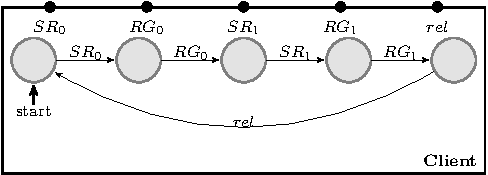
\includegraphics[scale=1.2]{compiledfigures/client-crop.pdf}
\caption{Client}
\label{fig:client}
\end{center}
\end{figure}

\begin{figure}[ht]
\begin{center}
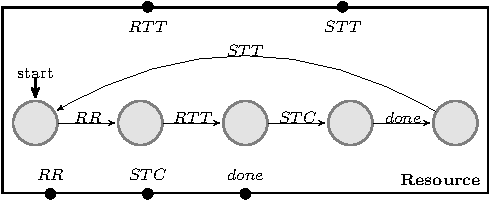
\includegraphics[scale=1.2]{compiledfigures/resource-crop.pdf}
\caption{Resource}
\label{fig:resourse}
\end{center}
\end{figure}

\begin{figure}[ht]
\begin{center}
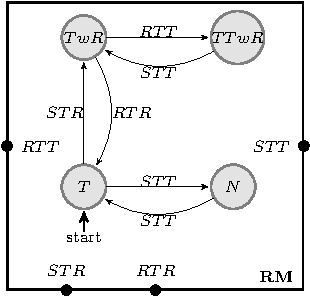
\includegraphics[scale=1.2]{compiledfigures/token-crop.pdf}
\caption{Token Resource Manager}
\label{fig:conflict-token}
\end{center}
\end{figure}

\begin{figure}[ht]
\begin{center}
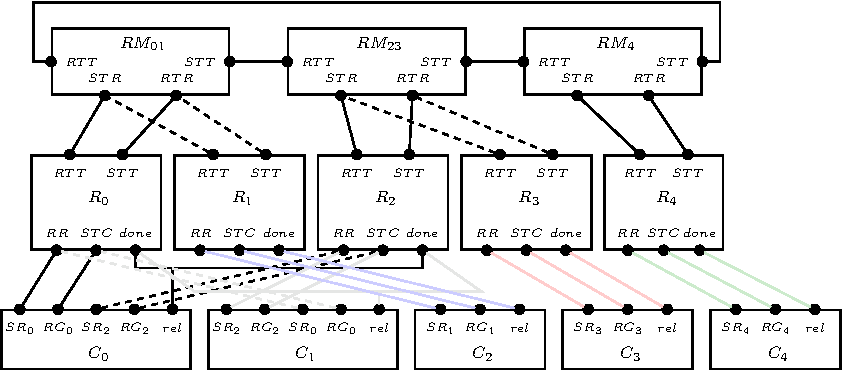
\includegraphics[scale=1.2]{compiledfigures/resourceallocation-crop.pdf}
\caption{Conflict-Resource Allocation System}
\label{fig:resourceallocation}
\end{center}
\end{figure}


**********************************************\\
Lesson 1: DFinder only global deadlock \\
5 clients and 5 resources \\
resourceMapping = {{0, 2}, {2, 0}, {1} , {3}, {4}};\\
conflictingResources = {{0, 1}, {2, 3}, {4}};\\
nbOfTokens = 3;\\\\


Local deadlock but not global deadlock \\
DFinder (deadlock-free)\\
however there exists a local deadlock (client0.RR, resource0.SR), whole system \\
**********************************************\\
Lesson 2: LALT more complete \\
5 clients and 5 resources; \\
resourceMapping = {{0, 2}, {0, 2}, {1} , {3}, {4}};\\
conflictingResources = {{0, 1}, {2, 3, 4}};\\
nbOfTokens = 2;\\

LALT no local and global deadlock \\
LLIN the system might contain deadlock \\
DFinder the system might contain deadlock\\
****************************************************
Lesson 3: Future work (a component may block forever, no local deadlock exists though)\\
Cannot find a subsystem s.t. when considered in isolation has a deadlock state (conspiracies)\\

5 clients and 5 resources; \\
resourceMapping = {{0, 1}, {1, 0}, {2} , {3}, {4}};\\
conflictingResources = {{0, 1}, {2, 3, 4}};\\
nbOfTokens = 2;\\

LALT no local and global deadlock \\
LLIN the system might contain deadlock  \\
DFinder the system might contain deadlock\\


\begin{table}
\centering
\begin{tabular}{| l | l | l | l |}
\hline
Size & \LAO & \LLin & D-Finder \\ \hline \hline
$10$ &          $148 s$ \\ \hline
$12$ &          $169 s$ \\ \hline
$14$ &          $189 s$ \\ \hline
$16$ &          $230 s$ \\ \hline
$18$ &          $254 s$  \\ \hline
$20$ &          $277 s$  \\ \hline 
$22$ &          $298 s$ \\ \hline 
$24$ &          $318 s$   \\ \hline 
$26$ &          $351 s$  \\ \hline 
$28$ &          $374 s$  \\ \hline
$30$ &          $430 s$   \\ \hline  
\end{tabular}
\caption{Benchmarks: Conflict-Resource Allocation}
\label{bench:resourceallocation}
\end{table}

TODO
\begin{itemize}
\item n clients, n resources , client i requests resource i, and n token 
\item number of states global system: $4^n \times 3^n \times 5^n$
\item maximum $\l$ is 2
\item \LAO linear w.r.t. n! although number of states is exponential w.r.t. n (12 components out of 3 * n), 23040000 states regardless of n
\item \LLin not complete (the system might contain deadlock)
\item D-Finder time limit (one hour) for n = 10. Try different combinations of partitions
\end{itemize}


